\documentclass[12pt]{article}
\usepackage{frExamplee}
\usepackage{booktabs}       % professional-quality tables
\usepackage{amsfonts}       % blackboard math symbols
\usepackage{amsmath}
\usepackage{enumitem}
\usepackage{listings}
\lstset{
    language=Python,
    basicstyle=\scriptsize\ttfamily,
    keywordstyle=\color{blue},
    commentstyle=\color{green!50!black},
    stringstyle=\color{red},
    showstringspaces=false,
    numbers=left,
    numberstyle=\footnotesize,
    numbersep=5pt,
    frame=single,
    breaklines=true,
    breakatwhitespace=true,
    tabsize=4,
    captionpos=b
}
\usepackage{amssymb}
\usepackage{graphicx}
\usepackage{csquotes}
\usepackage[backend=biber, style=ieee,]{biblatex}
\usepackage{setspace}
\usepackage[usenames, dvipsnames]{xcolor}
\usepackage{xspace}
\usepackage{caption}
\usepackage{subcaption}
\usepackage{multirow}
\usepackage{float}
\usepackage{wrapfig}
\usepackage{placeins}
\usepackage{algpseudocode}
\usepackage{algorithm}
\usepackage{algorithmicx}
\usepackage{hyperref}
\usepackage{setspace}
\usepackage{fancyhdr} 
\fancyhf{}
\cfoot{\thepage}
\pagestyle{fancy}
\renewcommand{\headrulewidth}{0pt}%

\addbibresource{FRtemplates/frExampleRefs.bib}
\title{An Investigation on the Thermal Diffusivity of Rubber}
\author{
Tony Wang \href{https://orcid.org/0009-0009-3015-7192}{
\includegraphics[height=12pt]{figure/orcid.png}}\\
\texttt{1009027447 | wangq330} \\
\texttt{tonyivt.wang@mail.utoronto.ca}\\
\And
Natasha Yang \href{https://orcid.org/12345}{
\includegraphics[height=12pt]{figure/orcid.png}}\\
\texttt{1008975575 | yangx315} \\
\texttt{nxy.yang@mail.utoronto.ca} \\
\And
Take Kawashima 
{
\includegraphics[height=12pt]{figure/orcid.png}}\\
\texttt{1008984315 | kawash11} \\
\texttt{take.kawashima@mail.utoronto.ca} \\
}
\begin{document}
\maketitle
\begin{abstract}
    This lab report investigates the thermal diffusivity constant, $m$, of a rubber cylinder by applying varying temperatures to its outer surface and measuring the inner surface temperature. The setup involves baths of hot and cold water where the rubber cylinder was swapped between these two baths to measure the change in rubber temperature with respect to time. The angular frequency, $\omega$ of the switching and the time delay between switching and the internal temperature changing, $\Delta t$ was experimentally found, enabling us to relate them and derive the thermal diffusivity constant of rubber as $(6.06 \pm 1.45) \times 10^{-7}\; [m^{2}/s]$. This value is within the accepted range of $0.89\times 10^{-7} \; [m^{2}/s]$ to $ 7.5\times 10^{-7}\; [m^{2}/s]$ reported in literature \autocite{article}, suggesting a successful experiment.
\end{abstract}

%------------------------------------------------------
% 7.41 * 10^-7 [m^2/s]
\section{Introduction}
Thermal diffusivity is a measure of the rate of heat transfer in an object. It is responsible for the determination of materials that offer the most efficient heat flow \autocite{onthermo}. Holding great significance, it is widely used in industries, from modeling heat transfer in combustion engines to microfluidics in computer cooling \autocite{thermoappli}. The governing equation in thermal diffusion is
\begin{equation}
    \frac{\partial T}{\partial t}=m\nabla^2T
    \label{eq:diffusion}
\end{equation}
where $m$ is the thermal diffusivity constant and $T$ is temperature, dependent on both time and position. In this experiment, our test specimen will be a long rubber cylinder, where we will be swapping it between a hot and cold water bath repeatedly. Hence, for simplicity we can parameterize (\ref{eq:diffusion}) in cylindrical coordinates \autocite{manuall}:
\begin{equation}
    \frac{\partial T}{\partial t}=m\left(\frac{\partial^2T}{\partial r^2}+\frac{1}{r}\frac{\partial T}{\partial r}\right)
    \label{eq:cylindrical}
\end{equation}
To find a simple solution to the partial differential equation, the temperature function can be modeled by separating itself into its position and time dependencies \autocite{manuall}:
\begin{equation}
    T(r,t)=R(r)\exp{(i\omega t)}
    \label{eq:seperation}
\end{equation}
where $\omega$ is the angular frequency. Substituting this solution into (\ref{eq:cylindrical}), we arrive at
\begin{equation}
    \frac{d^2R}{dr^2}+\frac{1}{r}\frac{dR}{dr}+\lambda^2R=0
    \label{eq:ode}
\end{equation}
where $\lambda^2=-\frac{i\omega}{m}$ which is a Bessel equation of order zero. A known solution to (\ref{eq:ode}) that satisfies the periodically changing boundary conditions is the order zero Bessel function \autocite{manuall}:
\begin{equation}
    J_0(z)=1-\frac{z^2}{2^2}+\frac{z^4}{2^24^2}-\frac{z^6}{2^24^26^2}+\dots
    \label{eq:bessel}
\end{equation}
where $z=\lambda r\in\mathbb{C}$ and the phase $\phi$ of the solution is:
\begin{equation}
    \tan\phi=\frac{\frac{x^2}{2^2}-\frac{x^6}{2^24^26^2}+\dots}{1-\frac{x^4}{2^24^2}+\dots}
    \label{eq:phase}
\end{equation}
where $x^2=\frac{r^2\omega}{m}$ \autocite{manuall}, or
\begin{equation}
    \phi=\arctan\frac{\frac{r^2\omega}{2^2m}-\frac{r^6\omega^3}{2^24^26^2m^3}+\dots}{1-\frac{r^4\omega^2}{2^24^2m^2}+\dots}
    \label{eq:phase1}
\end{equation}
Furthermore, the numerator and denominator of the above equation can be rewritten as: 
\begin{equation}
{\rm bei_0(\frac{r^2\omega}{m})} =\frac{r^2\omega}{2^2m}-\frac{r^6\omega^3}{2^24^26^2m^3}+\dots\text{ and }{\rm ber_{0}(\frac{r^2\omega}{m})} = 1-\frac{r^4\omega^2}{2^24^2m^2}+\dots
\label{eq:bb}
\end{equation}
where ${\rm bei_{0}}$ and ${\rm ber_{0}}$ are known as Kelvin Functions \autocite{Oldham2009}.

The phase difference between the bath temperature and the rubber temperature can be written as: 
\begin{equation}
    \Delta\phi = \phi_1 - \phi_2 = \omega\Delta t
    \label{eq:d_phi}
\end{equation}
where $\Delta t$ is the time delay between physically swapping the rubber between hot/cold water baths and the internal temperature responding to that change (reaching a maximum or minimum). Rearranging equation (\ref{eq:d_phi}), we obtain an expression for the time delay between when the thermometer was moved between different baths and when the measured temperature reached a peak or a trough:
\begin{equation}
    \Delta t=\frac{\Delta\phi}{\omega}=\frac{\phi_1-\phi_2}{\omega}
    \label{eq:dt}
\end{equation}
We use the $m$ dependence of $\phi$ to fit the relation, finding the least squares solution for thermal diffusivity.

\section{Experiment}
\subsection{Equipment and Uncertainties}
\begin{itemize}
    \item Hot plate
    \item Two glass jars
    \item Metal scissor lift
    \item Thermometer $(\pm 0.5\;^\circ C)$
    \item Burette stand
    \item Rubber Cylinder $(r_1=r_{\rm in}=6.5\pm0.005\;{ mm},\;r_2=r_{\rm out}=16\pm0.005\;{ mm})$
    \item Timer $(\pm 0.5\;s)$
    \item Digital caliper $(\pm 0.005\;mm)$
    \item Ice
\end{itemize}

\subsection{Apparatus}
\begin{figure}[h!]
    \centering
    \includegraphics[width=0.7\textwidth]{figure/Screenshot 2024-03-01 at 8.01.27 PM.png}
    \caption{Experimental apparatus with equipment labeled.}
    \label{fig:0}
\end{figure}

\subsection{Method} 
\subsubsection{Preparation}
\begin{enumerate}
    \item Fill one glass jar with water and place it on the hot plate. Turn on the hot plate and wait for the water to boil.
    \item Fill the other jar with mostly ice and add some water. Ensure that the heights of water in both jars are equal.
    \item Adjust the height of the cold water jar using the knob on the metal scissor lift to make both jars the same height.
    \item Measure the inner and outer radii of the rubber cylinder with caliper \autocite{manuall}.
\end{enumerate}
\subsubsection{Experiment}
\begin{enumerate}
    \item Begin by starting the timer and tightening the clamp on one end of the thermometer with the rubber cylinder attached while ensuring the rubber is mostly in the water without touching the bottom of the jar.
    \item Record the temperature change of the rubber cylinder until the end of the trial.
    \item After 240 seconds, switch the rubber cylinder to the other jar.
    \item Repeat step 3 six times to collect a sufficient amount of data.
    \item Repeat steps 1 to 4 five more times with different time intervals for switching the rubber cylinder (for 180s, 120s, 90s, 60s, and 30s instead of 240s) \autocite{manuall}. 
\end{enumerate}
\subsubsection{Data Processing}
The ultimate goal of this experiment is to use (\ref{eq:dt}) to numerically find the thermal diffusivity parameter, $m$ with the $\Delta t$ and $\omega$ values found in the lab. Since this relation is extremely complicated and computationally expensive to directly fit, mathematical simplifications can be made.

Given (\ref{eq:bb}), we can rewrite $\Delta\phi$ as
\begin{equation}
    \Delta\phi=\arctan\frac{{\rm bei_0}(x_1)}{{\rm ber_0}(x_1)}-\arctan\frac{{\rm bei_0}(x_2)}{{\rm ber_0}(x_2)}
    \label{eq:dphi}
\end{equation}
And relating this to (\ref{eq:dt}), we find an expression for $\Delta t(\omega)$:
\begin{equation}
    \Delta t(\omega)=\frac{1}{\omega}\left[\arctan\frac{{\rm bei_0}\left(r_1\sqrt{\frac{\omega}{m}}\right)}{{\rm ber_0}\left(r_1\sqrt{\frac{\omega}{m}}\right)}-\arctan\frac{{\rm bei_0}\left(r_2\sqrt{\frac{\omega}{m}}\right)}{{\rm ber_0}\left(r_2\sqrt{\frac{\omega}{m}}\right)}\right]
    \label{eq:beiber_0}
\end{equation}
To make this relation more practical to fit, we can utilize the Taylor Series expansions of 
(\ref{eq:beiber_0}) to get
\begin{equation}
    \arctan\frac{{\rm bei_0}\left(x\right)}{{\rm ber_0}\left(x\right)}\approx\frac{x^2}{4}-\frac{x^6}{576}+\frac{19x^{10}}{614400}+\dots
    \label{eq:atantaylor}
\end{equation}

Finally, with (\ref{eq:beiber_0}, \ref{eq:atantaylor}), we have
\begin{equation}
    \Delta t(\omega)\approx\left(\frac{r_1^2}{4m}-\frac{r_1^6\omega^2}{576m^3}+\frac{19r_1^{10}\omega^4}{614400m^5}\right)-\left(\frac{r_2^2}{4m}-\frac{r_2^6\omega^2}{576m^3}+\frac{19r_2^{10}\omega^4}{614400m^5}\right) + \Delta t_0
    \label{eq:final}
\end{equation}
which is consisted of polynomials and trivial to fit \autocite{wolframalpha}. We can add a constant upward shift $\Delta t_0$ (computed numerically) to account for solutions that are outside the range of $(-\pi/2,\pi/2)$.

\section{Data and Discussion}
Through one trial of the experiment, it is immediately evident that there is delay between the physical change of bath and the rubber temperature response (see Figure \ref{fig:1}). The overall temperature trend is reminiscent of a sinusoid, phase shifted by the time delay.

\begin{figure}[h!]
    \centering
    \includegraphics[width=0.7\textwidth]{figure/Screenshot 2024-03-01 at 2.13.34 PM.png}
    \caption{Change of hot/water baths graphed with the internal temperature of the rubber. It is evident that there is a substantial delay between the instantaneous change of the hot/cold bath square wave and the rubber temperature peak/troughs.}
    \label{fig:1}
\end{figure}

By fitting the Taylor Series in equation (\ref{eq:final}) with our $\Delta t$ and $\omega$ values collected in the experiment, we were able to numerically find $m$ based on $\Delta t$'s dependence on it.

As shown in Figure \ref{fig:fit}, we were able to get an excellent fit of the equation (\ref{eq:final}). Qualitatively, the entire range of the curve is within the uncertainty of each data point. The quantitative evaluation of goodness of fit supports the visual trend. With a $R^2$ very close to 1 and relatively small residuals, it is clear that the equation fitted models the data trends exceptionally well. Comparing the reduced $\chi^2$ value of $0.33$ with the critical value of $15.51$, it does not reject the model and we can again conclude that our fit is good and the uncertainties are reasonable.

\begin{figure}[h!]
    \centering
    \begin{subfigure}{0.82\textwidth}
        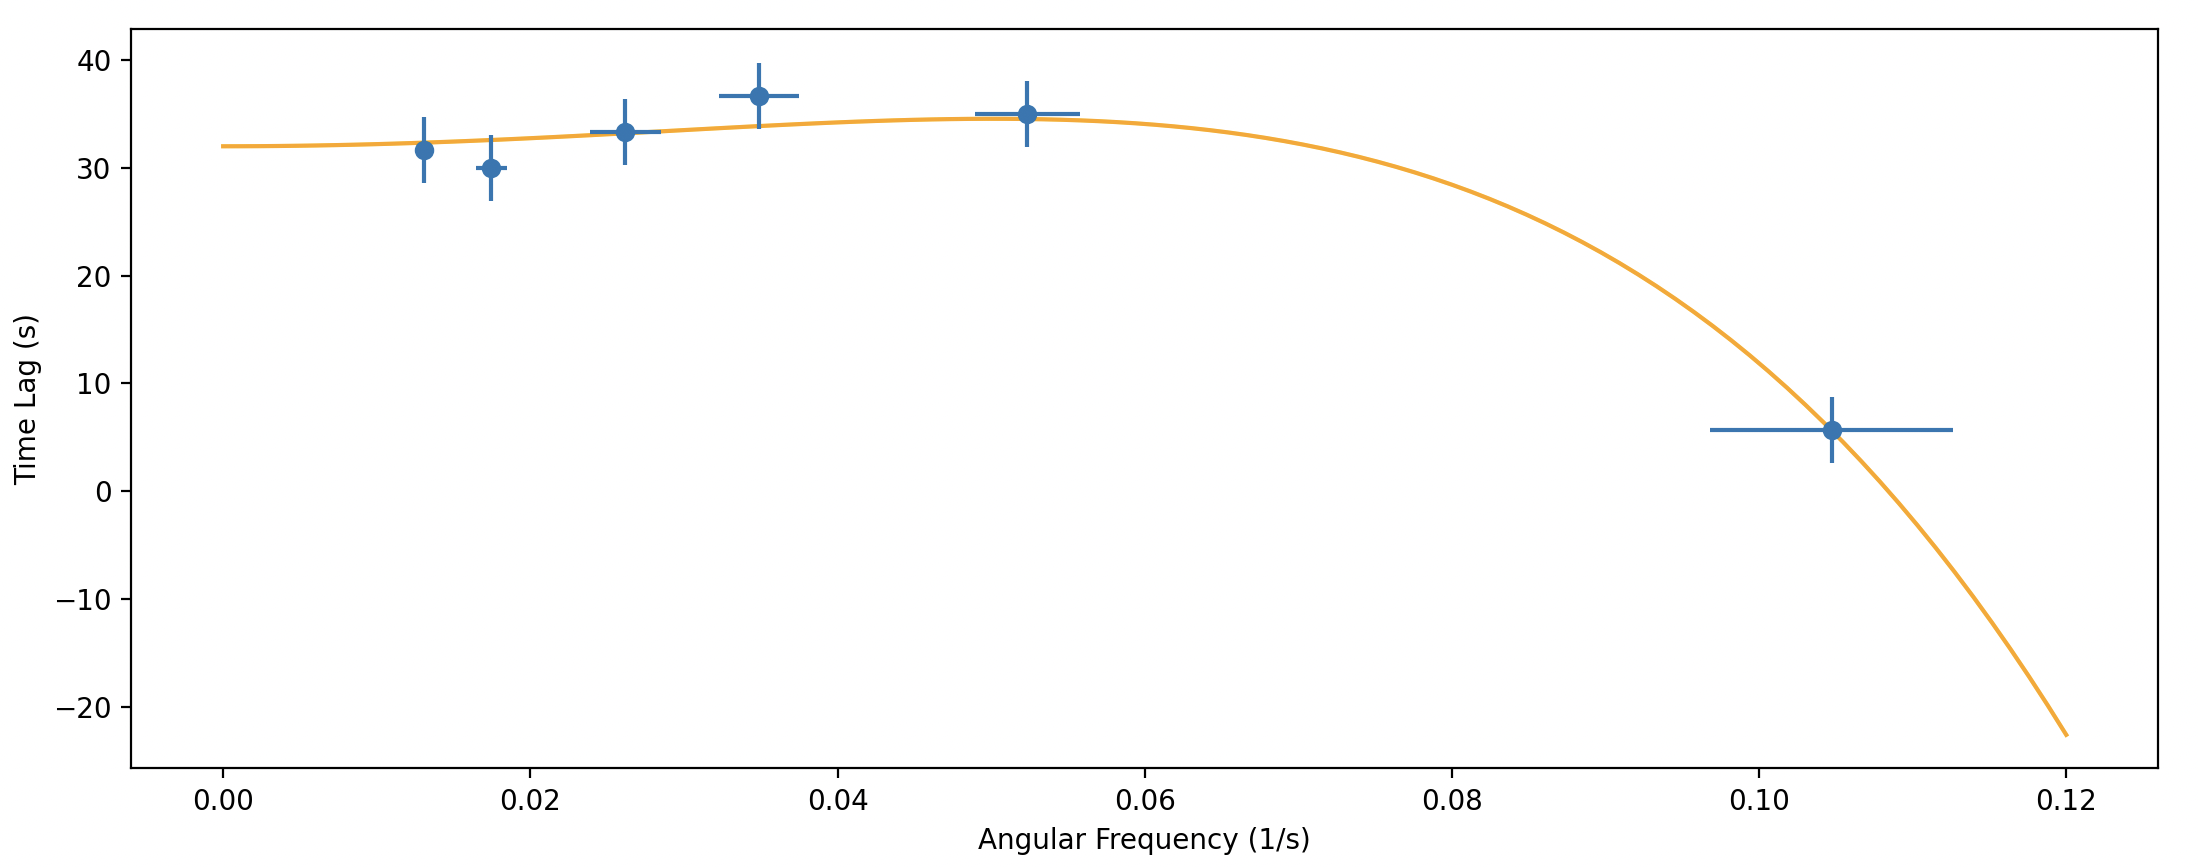
\includegraphics[width=\textwidth]{figure/data.png}
        \caption{Curve of best fit of (\ref{eq:final}). Note some error bars are too small to be shown.}
    \end{subfigure}
    \begin{subfigure}{0.9\textwidth}
        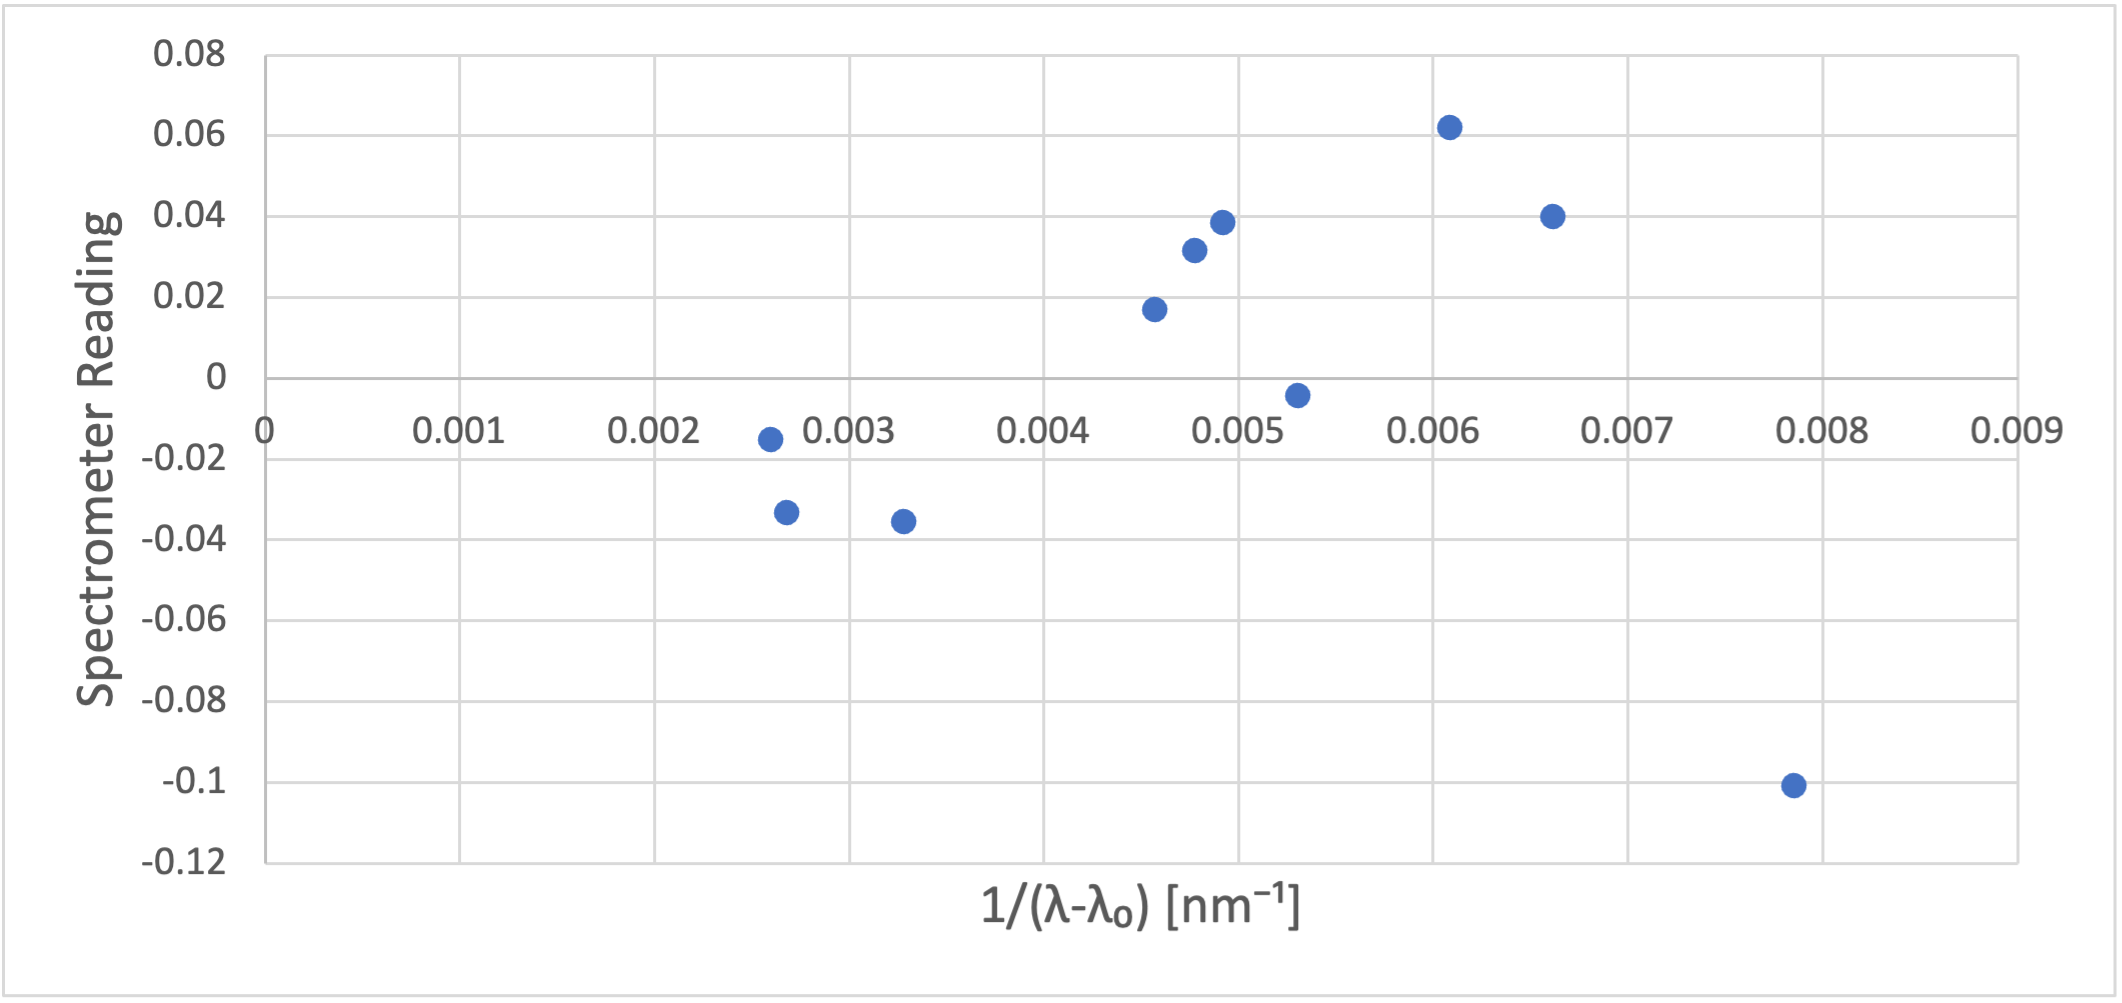
\includegraphics[width=\textwidth]{figure/residuals.png}
        \caption{Residual plot of of the curve fit of (\ref{eq:final}).}
    \end{subfigure}
    \caption{Fitting of $\Delta t(\omega)$ with error bars and residuals. The goodness of fit and error evaluation parameters are found to be: $R^2=0.98,\;\chi_{\rm reduced}^2=0.33,\;\chi_{\rm significance\;value}=0.05,\;\chi_{\rm critical\;value}=15.51$. Exact datapoint values can be found in Table \ref{table:1}.}
    \label{fig:fit}
\end{figure}

The thermal diffusivity of rubber was found to be: 
\begin{equation}
    \boxed{m_{\rm least-squares} = (6.06 \pm 1.45) \times 10^{-7}\; [m^{2}/s]}
    \label{eq:result}
\end{equation}
This number was computed with a least-squares upshift constant of $\Delta t_0=54.04\pm1.34\;[s]$, correcting the algorithm from only fitting to the default solution to the $\arctan$ function out of many.

The commonly used thermal diffusivity of rubber found by other researchers is $0.89\times 10^7\; [m^{2}/s]$ to $7.5\times 10^7\; [m^{2}/s]$ \autocite{article}. It verifies our findings, which is within this accepted range. However, the percentage uncertainty of our value (23.9\%), is still relatively large. This could be caused by a few sources of error. First, the Taylor series as outlined in (\ref{eq:final}) has a truncating error that scales with $O(\omega^6)$. Nevertheless, this should not be the largest source of error due to $\omega$ being less than 1. If this becomes a slight problem, simply using more terms in the Taylor Series will be a sufficient fix.

Another source of error came from the fundamental nature of the experiment design in that it required the manual switching of the rubber cylinder which causes the water bath switch to be inevitably non-instantaneous and results in inaccuracies that get propagated through data processing. It takes time to raise the rubber, shift it, and lower it back down into another water bath. In the future, if there are reasons that necessitate higher accuracy, an automated setup would be preferred over needing the involvement of humans.

In addition, rubber undergoes non-negligible thermal expansion and contraction when its temperatures vary significantly. For instance, when the rubber was bathed in hot water, reaching nearly 100 $^\circ C$, the outer diameter of the rubber sample was around 1 $mm$ larger than originally measured in ambient temperature as per our findings. Since the expression of $\Delta t(\omega)$ involves both the inner and outer radii, neglecting the change in size can have a nonzero influence on final results, though being hard to exactly quantify. To ensure higher accuracies, the radius should be propagated as a function of temperature instead of a set value.

Finally, uncertainties in reading the thermometer can be reduced if a digital one is used since the mercury thermometer does not have precise enough markings and involves human interpretation.

% \begin{figure}[h!]
%     \centering
%     \begin{subfigure}{0.47\textwidth}
%         \includegraphics[width=\textwidth]{figure/Screenshot 2024-03-01 at 2.13.34 PM.png}
%         \caption{Recorded data with slow switching frequency (high period, low angular frequency)}
%     \end{subfigure}
%     \begin{subfigure}{0.455\textwidth}
%         \includegraphics[width=\textwidth]{figure/Screenshot 2024-03-01 at 3.35.52 PM.png}
%         \caption{Recorded data with quick switching frequency (low period, high angular frequency)}
%         \label{fig:3b}
%     \end{subfigure}
%     \caption{Comparison of data accuracy between high and low hot/cold water bath switching frequency.}
%     \label{fig:error}
% \end{figure}

\section{Conclusion}
In this experiment, the thermal diffusivity constant of the rubber cylinder was investigated. The experiment consisted of alternating the rubber cylinder between hot and cold water baths and measuring the inner surface temperature change of the rubber cylinder. The resulting data was then used to obtain a periodic graph as seen in Figure \ref{fig:1}. Subsequently, the temperature change ($\Delta t$) as a function of angular frequency ($\omega$) was fitted with equation (\ref{eq:final}), a Taylor Series expansion of equation (\ref{eq:dt}) to obtain a thermal diffusivity constant of rubber cylinder as $(6.06 \pm 1.45) \times 10^{-7}\; [m^{2}/s]$.

This value, when considering uncertainties, is consistent with the range of values reported in current literature, $0.89\times 10^7\; [m^{2}/s]$ to $7.5\times 10^7\; [m^{2}/s]$ \autocite{article}, with evidence of accuracy supported by the residual plot seen in Figure \ref{fig:fit} with an excellent $R^2$ value of 0.98 and satisfactory reduced $\chi^2$ value. Despite the agreement, however, some uncertainties such as the time it takes to switch rubber between baths and the thermal expansion of rubber may have influenced the accuracy of the result. Future experiments can reduce this error by finding a better method to switch the rubber between the baths and taking the thermal expansion of materials into consideration.


\newpage
\printbibliography


\section*{Appendix}
\subsection*{Data}
\begin{table}[h!]
\centering
\caption{Experimental Data with Uncertainties}
\begin{tabular}{S[table-format=2.3] S[table-format=2.3(2)]} 
\toprule
$\omega\;[1/s]$ & $\Delta t\;[s]$ \\ 
\midrule
0.0131 $\pm$ 0.0005 &  31.67 $\pm$ 3.05  \\ 
0.0175 $\pm$ 0.0010 & 30.00 $\pm$ 3.05 \\ 
0.0262 $\pm$ 0.0023 &  33.33 $\pm$ 3.05  \\ 
0.0349 $\pm$ 0.0026 & 36.67 $\pm$ 3.05 \\ 
0.0524 $\pm$ 0.0034 &  35.00 $\pm$ 3.05  \\ 
0.1047 $\pm$ 0.0079 & 5.67 $\pm$ 3.05 \\
\bottomrule
\end{tabular}
\label{table:1}
\end{table}
\subsection*{Uncertainties Propagation}
\textbf{Uncertainties for $\omega$}\\
\begin{align*}
    \omega &= \frac{1}{T}\\
    \sigma_\omega &= \left| \frac{\partial \omega}{\partial T} \right| \sigma_T\\
    \sigma_\omega &= \left| -\frac{1}{T^2} \right| \sigma_T\\
    \sigma_\omega &= \frac{1}{T^2} \sigma_T
\end{align*}

\textbf{Uncertainties for $\Delta t$}\\
We estimate the uncertainty of the time delay between water bath switches as a sum of the timer uncertainty and human error, where human error is dominant and estimated.
$$\sigma_{\Delta t}=\sigma_\epsilon+\sigma_t=3+0.05\;[s]$$

\textbf{Other Uncertainties related to }$\Delta t(\omega)$\\
Note that since the curve is fitted with \texttt{scipy.optimize}, uncertainties of fitting parameters and variables are numerically propagated with \texttt{scipy} as shown below. The error truncation of the series is also considered.

\newpage
\subsection*{Plotting and Goodness of Fit Code}
\textbf{For Figure }\ref{fig:1}
\begin{lstlisting}
import argparse
import numpy as np
import pandas as pd
import matplotlib.pyplot as plt
from scipy.optimize import curve_fit

def parse_args():
    parser = argparse.ArgumentParser(description="Fit sinusoidal function and plot square wave.")
    parser.add_argument("input_csv", help="Input CSV file")
    parser.add_argument("--start_high", action="store_true", help="Start square wave with high temperature")
    parser.add_argument("--period", type=float, required=True, help="Period of the square wave in seconds")
    return parser.parse_args()

def square_wave(t, start_high, period):
    phase_shift = 0 if start_high else period / 2
    return np.where((t + phase_shift) % period < period / 2, 100, 0)

def sinusoidal_func(t, A, omega, phi, offset):
    return A * np.sin(omega * t + phi) + offset

def fit_and_plot(input_csv, start_high, period):
    data = pd.read_csv(input_csv, header=None, names=["Time", "Temperature"], skipinitialspace=True)
    data.dropna(inplace=True)
    plt.plot(data["Time"], data["Temperature"], 'bo', label="Data")
    initial_guess = [50, 2 * np.pi / period, 0, 0]
    params, covariance = curve_fit(sinusoidal_func, data["Time"], data["Temperature"], p0=initial_guess)
    fitted_curve = sinusoidal_func(data["Time"], *params)
    plt.plot(data["Time"], fitted_curve, 'b-', label="Sinusoidal Fit")
    square_wave_values = square_wave(data["Time"], start_high, period)
    plt.plot(data["Time"], square_wave_values, 'orange', label="Square Wave")
    angular_frequency = params[1]
    plt.text(0.95, 0.05, f"Angular Frequency: {angular_frequency:.4f} rad/s", transform=plt.gca().transAxes, ha='right')
    plt.legend()
    plt.xlabel("Time (s)")
    plt.ylabel("Temperature $(^\circ C)$")
    plt.show()

def main():
    args = parse_args()
    fit_and_plot(args.input_csv, args.start_high, args.period)

if __name__ == "__main__":
    main()
\end{lstlisting}

\newpage
\textbf{For Figure }\ref{fig:fit}
\begin{lstlisting}
import scipy.optimize as optimize
import numpy as np
import matplotlib.pyplot as plt

w = np.array([0.01308996939, 0.01745329252, 0.02617993878, 0.03490658504, 0.05235987756, 0.1047197551])
uncertainty_w = np.array([0.0005, 0.0010, 0.0023, 0.0026, 0.0034, 0.0079])
d_t = np.array([31.66666667, 30, 33.33333333, 36.66666667, 35, 5.66666667])
uncertainty_dt = np.array([3.05, 3.05, 3.05, 3.05, 3.05, 3.05])
r1 = 6.5/1000/2
uncertainty_r1 = 0.000005
r2 = 16/1000/2
uncertainty_r2 = 0.000005

def T(w, m):
    T1 = (r1**2)/(4*m) - (r1**6) * (w**2) / (576 * m**3) + 19 * (r1**10) * (w**4) / (614400 * m**5)
    T2 = (r2**2)/(4*m) - (r2**6) * (w**2) / (576 * m**3) + 19 * (r2**10) * (w**4) / (614400 * m**5)
    return T1 - T2 + 54

m_opt, pcov = optimize.curve_fit(T, w, d_t, sigma=uncertainty_dt, absolute_sigma=True)  # Include errors
print(m_opt)

y_fit = T(w, m_opt)
residuals = d_t - y_fit
ss_res = np.sum(residuals**2)  
ss_tot = np.sum((d_t - np.mean(d_t))**2) 
r_squared = 1 - (ss_res / ss_tot)
print("R-squared:", r_squared)

chi_squared = np.sum((residuals / uncertainty_dt)**2)
dof = len(w) - 1  # Degrees of freedom
reduced_chi_squared = chi_squared / dof
print("Reduced chi-squared:", reduced_chi_squared)

x = np.linspace(0, 0.12, 100)
plt.plot(x, T(x, m_opt), color='orange')  # Fitted curve in orange
plt.errorbar(w, d_t, xerr=uncertainty_w, yerr=uncertainty_dt, fmt='o')  # Error bars
plt.xlabel('Angular Frequency (1/s)')
plt.ylabel('Time Lag (s)')

plt.figure()  
plt.scatter(w, residuals)  # Plot residuals against ω
plt.axhline(0, color='gray', linestyle='--')  
plt.xlabel('Residuals of Angular Frequency (1/s)')  # Change label
plt.ylabel('Residuals of Time Lag (s)')  # Change label

ax = plt.gca()  # Get the current axis
textstr = f"\nR-squared: {r_squared:.2f}\nReduced chi-squared: {reduced_chi_squared:.2f}"  # Include fitted parameter
props = dict(color="black", fontsize=10)
ax.text(0.05, 0.05, textstr, transform=ax.transAxes, fontsize=10, verticalalignment="bottom", bbox=dict(facecolor='white', edgecolor='black'))

plt.show()
\end{lstlisting}

\end{document}